% Compile with pdflatex.

\documentclass{ISIS}
\usepackage{amsfonts}
\usepackage{multirow}
\usepackage{xcolor}% http://ctan.org/pkg/xcolor

\confyear{2021}
\confnumber{22nd}
\setarticlestartpagenumber{1}

%--------------------------------------------
\def\sqPDF#1#2{0 0 m #1 0 l #1 #1 l 0 #1 l h}
\def\trianPDF#1#2{0 0 m #1 0 l #2 4.5 l h}
\def\uptrianPDF#1#2{#2 0 m #1 4.5 l 0 4.5 l h}
\def\circPDF#1#2{#1 0 0 #1 #2 #2 cm .1 w .5 0 m
	.5 .276 .276 .5 0 .5 c -.276 .5 -.5 .276 -.5 0 c
	-.5 -.276 -.276 -.5 0 -.5 c .276 -.5 .5 -.276 .5 0 c h}
\def\diaPDF#1#2{#2 0 m #1 #2 l #2 #1 l 0 #2 l h}

\def\credCOLOR   {.54 .14 0}
\def\cblueCOLOR  {.06 .3 .54}
\def\cgreenCOLOR {0 .54 0}
\def\cDCCOLOR   {0 .84 .93}
\def\cHCCOLOR   {.80 0 .99}
\def\cRCCOLOR   {0 0 0}
\def\cTKCOLOR   {.75 .75 0}

\def\genbox#1#2#3#4#5#6{% #1=0/1, #2=color, #3=shape, #4=raise, #5=width, #6=width/2
	\leavevmode\raise#4bp\hbox to#5bp{\vrule height#5bp depth0bp width0bp
		\pdfliteral{q .5 w \csname #2COLOR\endcsname\space RG
			\csname #3PDF\endcsname{#5}{#6} S Q
			\ifx1#1 q \csname #2COLOR\endcsname\space rg 
			\csname #3PDF\endcsname{#5}{#6} f Q\fi}\hss}}

% shape     raise width  width/2
\def\sqbox      #1#2{\genbox{#1}{#2}  {sq}       {0}   {4.5}  {2.25}}
\def\trianbox   #1#2{\genbox{#1}{#2}  {trian}    {0}   {5}    {2.5}}
\def\uptrianbox #1#2{\genbox{#1}{#2}  {uptrian}  {0}   {5}    {2.5}}
\def\circbox    #1#2{\genbox{#1}{#2}  {circ}     {0}   {5}    {2.5}}
\def\diabox     #1#2{\genbox{#1}{#2}  {dia}      {-.5} {6}    {3}}

%% usage:

%squares: \sqbox0{cgreen}, \sqbox1{cred}, \sqbox0{cblue}.
%
%triangles: \trianbox0{cgreen}, \trianbox1{cred}, \trianbox0{cblue}.
%
%triangles: \uptrianbox0{cgreen}, \uptrianbox1{cred}, \uptrianbox0{cblue}.
%
%circles: \circbox0{cgreen}, \circbox1{cred}, \circbox0{cblue}.
%
%diamonds: \diabox0{cgreen}, \diabox1{cred}, \diabox0{cblue}.
%--------------------------------------------
%
\usepackage{stackengine}
\newcommand\xrowht[2][0]{\addstackgap[.5\dimexpr#2\relax]{\vphantom{#1}}}
%--------------------------------------------

\allowdisplaybreaks

\begin{document}
\title{\begin{center}A Dimension Reduction Technique to Classify Upper Arm Gym-Workouts in Realtime with TinyML\end{center}}
\author{Ho-Jin Jung\inst{1}, Changjae Lee\inst{2}, and Han Ul Yoon\inst{2}}
\institute{Division of Computer and Telecommunication Engineering, Yonsei University (Mirae)\\Wonju 26493, Korea \\ \inst{2}Division of Software, Yonsei University (Mirae)\\ Wonju 26493, Korea}
\email{\{hojinj,cjlee7128,huyoon\}@yonsei.ac.kr}

\begin{abstract}
%This paper proposes a dimension reduction   system for classifying upper arm gym-workouts based on biopotential and kinematic data. The key idea is to plot the feature of workout data in the 2D coordinate. If it’s similar workout, it’ll be marked close, otherwise it’s far. To achieve this, our system learns to map high-dimensional data to two dimension in which the reduced data can be plotted and clustered. Then, the sample is able to be mapped on the reduced dimension coordinate. After calculating the distance between the mapped sample and each group’s centroid, our system predicts which group it belongs to. We show the performance of classification on biceps brachii workouts and triceps brachii workouts.
Biopotentials are typically measured by multichannel probes and recorded as time-series data. Accordingly, the measured biopotentials have high dimensionality which impedes to build a fast machine classifier using an affordable system, i.e., TinyML. In this paper, we propose a dimension reduction technique for multichannel surface EMG time series data being measured during various upper arm gym-workouts. The key idea of our approach is to utilize t-stochastic neighbor embedding as a tool for the dimension reduction of a feature space to where data samples belong. Then, the data samples in the reduced feature space are grouped, labeled, and represented as Gaussian distributions according to workout names. 
%
Lastly, we train a neural network to functionally approximate the above-mentioned dimension reduction process, which eventually enables us to classify a newly given data sample based on Mahalanobis distance to each workout group.
%
For upper arm gym-workout classification, under the proposed approach, the result shows the accuracy of 85.25 percent in terms of macro-precision.       
\end{abstract}

\begin{keywords}
Upper Arm Gym-Workout Classification, Dimensionality Reduction, Surface EMG-based Classification 
\end{keywords}
\maketitle


\section{Introduction}
%
Nowadays, time-series data analysis plays essential roles in a broad range of field. By analyzing the time-series data, for example, we can predict a house electricity consumption with quarterly/yearly record, diagnosis a heart difficiency based on ECG, forecast a stock market, and so on. Accordingly, many studies have been undertaken to develop and innovate the time-series data analysis techniques, e.g., parametric time-series identification~\cite{Astrom}, dynamic time warping-based pattern recognition~\cite{Berndt}, various data mining approaches~\cite{TcFu}, etc.   

In our previous study presented in~\cite{JHYoo}, we defined a correct workout as ``stimulating correct target muscles while performing a timely sequence of correct motion primitives.'' We also showed that upper arm gym-workouts could be classified successfully via convolutional neural network by merging surface EMG~(sEMG) data with an elbow joint angle data and visualizing it as an image. In this paper, we proposes a dimension reduction technique to solve the same upper arm gym-workouts classification problem. This study has been initiated to investigate a feasibility of building an affordable AI-based home trainer using TinyML. In the proposed technique, t-stochastic neighbor embedding~(t-SNE) serves as a tool to reduce a feature space dimensionality. In the reduced feature space, the sample data of each workout group are represented as Gaussian distributions. 
%
The outcomes from the t-SNE will be eventually used to train a neural network~(NN) to functionally approximate a relationship between a high dimensional input data and a t-SNE output. Consequently, when a new workout data is given, it passes through the trained NN, and the output can be classified based on Mahalanobis distance to each workout group.
%

The rest of paper is organized as follows. In Section 2, we introduce data measurement, data pre-processing, and a dimensionality reduction technique as well as a corresponding classifier system design. In Section 3, the evaluation results for the proposed approach are presented. Section 4 will be the conclusion of this paper and a future direction will be discussed shortly. 


\section{Methods}

\subsection{Data measurement}
A professional trainer was recruited to measure upper arm gym-workout data. Four different workouts were demonstrated by the trainer, i.e., dumbbell curl~(DC), hammer curl~(HC), reverse curl~(RC), and triceps kickback~(TK). DC, HC, and RC were chosen to stimulate biceps brachii muscles whereas TC targeted triceps brachii muscles. An armband type sEMG sensor (Myo Armband, Thalmic Labs, Brooklyn, NY) was mounted on the trainer's right upper arm. The 8 sEMG channels were deployed as channel 1 through 3 on biceps brachii area and channel 5 through 7 on triceps brachii. Channel 4 and 8 were located on boundaries between biceps and triceps brachii. In addition, an elbow joint angle was measured by a RGB-d camera~(Kinect v2 for Windows, Microsoft, Redmond, WA) and a Vitruvius framework~(Vitruvius Kinect, LightBuzz Inc., New York, NY). 

\subsection{Data acquisition and pre-processing}
For data acquisition, sampling time was set to 20ms and the trainer was instructed to rhythmically demonstrate one repetition during 1600 ms basis; therefore, 80 data samples were recorded per one repetition. A time stamp was increased rowwise. The data field for one data sample in a row was {\texttt{[sEMGch(1:8), elbow\_joint\_angle]}} in a form of MATLAB-like notation. To prevent muscle fatigue, one set was limited to 20 repetitions. Three sets were performed for each workout types. Consequently, a total 240 data samples~(20 repetitions $\times$ 3 sets $\times$ 4 workout types) were obtained from the trainer's demonstration. The obtained data set was pre-processed by following steps:
\begin{enumerate}
	\item Take the absolute value for the obtained data set.
	\item Apply a moving average filter. A window size was set to 10 time steps.
	\item Integrate the filtered data. An interval size was set to 5 time steps.
	\item Perform inter-channel normalization. By completing upto this step, we obtain a matrix whose size is 9 by 16.
	\item Flatten the above matrix; hence, a data sample for one repetition was converted into a vector in $\mathbb{R}^{144 \times 1}$. 
\end{enumerate}  
For more details, please refer to our previous study disseminated in~\cite{JHYoo}.

%The data consist of EMG signal and elbow joint angle. The data used in [4] consisted of EMG signals and elbow joint angles measured during four upper gym-workout Dumbbell curl (DC), Hammer curl (HC), Reverse curl (RC), and Triceps kickback (TK) with different bicep and triceps usage ratios. DC, HC, and RC target biceps brachii training and TK targets triceps brachii training. EMG signal consisting of 8 channels was measured via armband electromyography sensor (Myo armband). The Myoarmband was mounted on the right side and the biceps brachii area for ch.1~4 and the triceps brachii area for ch.5~8. Elbow joint angle value got from the angle between the right upper arm and the right lower arm by measurement via RGBD camera (Kinect-V2). The data acquisition format is [ch1:8, elbow\_joint\_angle] and consists of 1600ms by measuring 80 times at 20ms intervals. A total of 240 data were obtained by performing 60 times per workout in the same way as above. 

\subsection{Dimension reduction and workout group representation}
Recall that we converted total  240 data samples into the flattened vector which consisted of 144 features. The high dimensionality of the resulting flattened vector indeed impeded to design an affordable AI-based home trainer or exercise monitoring system. To address this issue, we utilized t-SNE to reduce a feature space dimensionality with the following purposes:
%
\begin{itemize}
	\item We wanted to stochastically project all data samples onto a visible dimension.   
	\item We wanted to investigate whether data samples are separable according to their workout groups(types).
	\item If separable, we wanted to find a way to represent workout groups, e.g., separating hyperplanes, mean and covariance, etc. 
\end{itemize}

Figure \ref{fig:tSNE_gauss} illustrates all data samples projected onto two dimensional feature space and workout groups represented by Gaussian distributions. From Fig. \ref{fig:tSNE_gauss}(left), we could observe that data samples could be separable according to their workout groups. Also, without a loss of generality, we could conclude that it would be better way to represent workout groups as Gaussian distributions as shown in Fig. \ref{fig:tSNE_gauss}(right) than linearly separating hyperplanes. Of course, kernel estimation-based approaches, for instance, support vector machine, could yield outperforming nonlinear decision boundaries; however, we note that the simpler method was preferred by considering affordability. The mean $\mu_i$ and covariance matrix $\Sigma_i$ were calculated from the samples belong to each workout group.     

\begin{figure}[!b]
	\begin{center}
		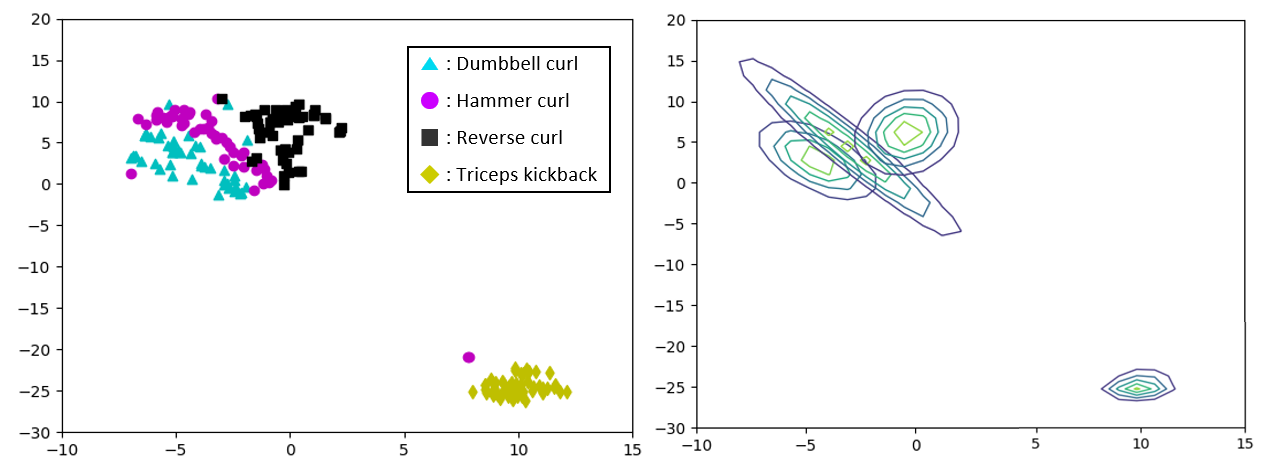
\includegraphics[width=0.9\linewidth]{Figure1}
		\caption{All data samples projected onto two dimensional feature space~(left)\\ and workout groups represented by Gaussian distributions~(right).}\label{fig:tSNE_gauss}
	\end{center}
	\vskip -1pc
\end{figure}

\subsection{Training a neural network and classifying a new workout data}
{ \color{black}{ If the t-SNE is needed to be performed for every newly given data sample, then the entire workout classification process would be severely down-speeded. Therefore, given the flattened input vectors and the t-SNE outputs, we trained a NN to functionally approximate the t-SNE, which in turn serves as a surrogate system for the t-SNE. After training the NN, workout classification could be processed for an upcoming flattened input vectors as follows: } }

\begin{enumerate}
	\item Pass the flattened input vector of $\mathbb{R}^{144 \times 1}$ through the trained NN and obtain the corresponding output of $\mathbb{R}^{2 \times 1}$.
	\item (optional) Plot the output in the reduced feature space.
	\item Calculate a Mahalanobis distances to each workout group.
	\item The new data belong to the workout group which returns the minimum Mahalanobis distance.
\end{enumerate} 

A total 240 data samples was divided into 192:24:24 samples as training:validation:test sets. To evaluate proposed classification approach, we performed upper arm gym-workout classification twenty-five times by pseudo-randomizing the test set, which corresponded to 150 classification test for each workout group.   

%If the information of the workout data feature can be plotted in the coordinate, biceps brachii workout probably are so far from triceps brachii workout. In contrast, distances between biceps brachii workouts are relatively closed. Since the dimension of the data is high, they cannot be plotted in two-dimension coordinate. To address this problem, the data need to be mapped the two-dimension via t-NSE. t-SNE transforms high dimensional data to low dimensional embedding space. The method compares between similarity of original space and similarity of embedding space via t-distribution [5]. After processing all the workout data, we can see that each group is well clustered. (See figure 1 for the full details). In t-SNE, the result is completely new whenever the input value changes. In other words, t-SNE does not obtain a result by learning only additional sample data. It remaps all data. Therefore, it is a large overhead to use t-SNE every time to obtain a cluster. Therefore, for learning to map the high dimensional value to the reduced dimension, neural network (NN) is employed. In other words, NN learns the result distribution of t-SNE. The NN uses 144-dimension input vector, 2-dimension output vector and loss function using Mean Square Error. A total of 240 data are divided in an 8(train):1(validation):1(test) ratio. Then, the data are composed of 48 * 4 = 192 train data, 6 * 4 = 24 validation data and 6 * 4 = 24 test data, and only 216 data excluding test data are used for train and validation of the NN. The test data will be used in the final stage of the classification. 
%We put the sample as an input of the NN and map it into a two-dimensional coordinate in the way described above. After that, our system can classify it to the closest group. The numeric value which obtained two-dimension coordinate via t-SNE are not valid, that is, to calculate between the sample and each group’s centroid using general Euclidean distance is not correct. But, the distribution of data is valid to be used as a criterion. Therefore, we employ the Mahalanobis distance that calculates using the average of data distribution and covariance matrix of data distribution [6]. 

\newcommand{\mcircle}{{\color{magenta}{$\bullet$}}}
\section{Results and Discussion}
%
Table \ref{tbl:result} presents a confusion matrix of upper arm gym-workout classification results. As it could be expected by observing Fig. \ref{fig:tSNE_gauss}, the correct prediction for TK outperformed all biceps brachii workouts. The largest Type I error occurred when ground truth was DC but prediction was HC. Among biceps brachii workouts, RC showed the most correct prediction. The resulting workout classification accuracy was 85.25 percent in terms of macro-precision.
% \trianbox1{cDC}  \circbox1{cHC}  \sqbox1{cRC} \diabox1{cTK}


\begin{table}[!b]
	\centering
	\caption{A confusion matrix of upper arm gym-workout classification results} \label{tbl:result}
\begin{tabular}{cc|c|c|c|c|l}	
	\cline{3-6}
	& & \multicolumn{4}{ c| }{Prediction} \\ \cline{3-6}
	& & DC(\trianbox1{cDC}) & HC(\circbox1{cHC}) & RC(\sqbox1{cRC}) & TK(\diabox1{cTK}) \xrowht{20pt} \\ \cline{1-6}
	\multicolumn{1}{ |c  }{\multirow{4}{*}{ \vspace{-4.0em}Ground truth} } & 
	\multicolumn{1}{ |c| }{DC(\trianbox1{cDC})} & \cellcolor[rgb]{.93,.49,.19} 104 & \cellcolor[rgb]{.97,.80,.68} 46 & \cellcolor[rgb]{.97,.80,.68} 0 & \cellcolor[rgb]{.97,.80,.68} 0 &  \xrowht{20pt} \\  \cline{2-6} 
	\multicolumn{1}{ |c  }{}  & 
	\multicolumn{1}{ |c| }{HC(\circbox1{cHC})} & \cellcolor[rgb]{.97,.80,.68} 13 & \cellcolor[rgb]{.93,.49,.19} 118 & \cellcolor[rgb]{.97,.80,.68} 17 & \cellcolor[rgb]{.97,.80,.68} 2 & \xrowht{20pt} \\ \cline{2-6} 
	\multicolumn{1}{ |c  }{}  &
	\multicolumn{1}{ |c| }{RC(\sqbox1{cRC})} & \cellcolor[rgb]{.97,.80,.68} 0 & \cellcolor[rgb]{.97,.80,.68} 18 & \cellcolor[rgb]{.93,.49,.19}  132 & \cellcolor[rgb]{.97,.80,.68} 0 & \xrowht{20pt} \\ \cline{2-6}  
	\multicolumn{1}{ |c  }{}  &
	\multicolumn{1}{ |c| }{TK(\diabox1{cTK})} & \cellcolor[rgb]{.97,.80,.68} 0 & \cellcolor[rgb]{.97,.80,.68} 0 & \cellcolor[rgb]{.97,.80,.68} 0 & \cellcolor[rgb]{.93,.49,.19} 150 & \xrowht{20pt}  \\ \cline{1-6} 
\end{tabular}
\end{table}

%\begin{figure}[!b]
%\begin{center}
%\includegraphics[width=\linewidth]{Table1}
%\caption{Result of final classification}\label{tbl:result}
%\end{center}
%\vskip -1pc
%\end{figure}



%\vspace{5.0em}
%With the introduced method in section 2, we performed the train/validation of the NN and the test of classification independently 25 times. The table 1 represents a confusion matrix of final classification result, which shows that macro-precision is 85.25%, macro-recall is 84.00%, macro-f1 is 84.15% and accuracy is 84.00%. Classification using time series data which is composed of EMG and elbow joint angle leads to satisfactory accuracy. Our system correctly classifies between biceps brachii workout and triceps brachii workout, and it can well classify between each biceps brachii workout too.

\section{Conclusion}
%
Throughout this paper, we proposed the dimension reduction technique to classify upper arm gym-workouts. The proposed approach first projected the high dimensional features onto two dimensional feature space by utilizing the t-SNE. After reducing the dimensionality of the feature space, data samples were represented by Gaussian distributions in two dimensional feature space. The functionality of the t-SNE was approximated by a neural network, which in turn allowed us to classify a newly given data sample based on the Mahalanobis distance from each group. As future works, this study will be culminated to the development of an affordable AI-based home training system. 


\subsection*{Acknowledgments}
This research was supported by the Ministry of Science and ICT, Korea, under the National
Program for ``Excellence in SW (Grant Number: 2019-0-01219)'' supervised by the Institute of
Information and Communications Technology Planning and evaluation (IITP).

\begin{reference}
\bibitem{Astrom} K. J. Astrom, ``On the choice of sampling rates in parametric identification of time series,'' \textit{Information Sciences}, vol.1, no. 3, pp. 273–278, July 1969.

\bibitem{Berndt} D. J. Berndt and J. Clifford, ``Using dynamic time warping to find patterns in time series,'' \textit{Proc. of the 3rd International Conference on Knowledge Discovery and Data Mining}, pp. 359–370, July 1994.

\bibitem{TcFu} T.-C. Fu, ``A review on time series data mining,'' \textit{Engineering Applications of Artificial Intelligence}, vol. 24, no. 1, pp. 164-181, February 2011. 

\bibitem{JHYoo} J.-H. Yoo, H.-J. Jung, and H.-U. Yoon, ``AI-based personal exercise monitoring system for biomechanical efficiency analysis and injury prevention,'' \textit{Journal of Korean Institute of Intelligent System}, vol. 31, no. 4, pp. 279-286, August 2021. 

\bibitem{Hinton} L. van der Maaten and G. Hinton, ``Visualizing Data using t-SNE,'' \textit{Journal of Machine Learning Research}, vol. 9, pp. 2579-2605, November 2008. 

%\bibitem{Vaswani} A. Vaswani, N. Shazeer, N. Parmar, J. Uszkoreit, L. Jones, A. Gomez, L. Kaiser, and I. Polosukhin, ``Attention is all you need,'' \textit{In Advances in Neural Information Processing Systems}, pp. 6000-6010, 2017. 

%\bibitem{Sutskever} I. Sutskever, O. Vinyals, and Q. V. Le, ``Sequence to sequence learning with neural networks,'' \textit{In Advances in Neural Information Processing Systems}, pp. 3104-3112, 2014. 

%저널
%\bibitem{BaCh} R. C. Baker and B. Charlie, ``Nonlinear unstable systems,'' \textit{International Journal of Control}, vol. 23, no. 4, pp. 123-145, May 1989.

%매거진
%\bibitem{Hong} G.-D. Hong, ``Linear controllable systems,'' \textit{Nature}, vol. 135, no. 5, pp. 18-27, July 1990.

%트랜잭션(저널)
%\bibitem{HongKim} K. S. Hong and C. S. Kim, ``Linear stable systems,'' \textit{IEEE Trans. on Automatic Control}, vol. 33, no. 3, pp. 1234-1245, December 1993.

%프로시딩
%\bibitem{ShFiDu} Z. Shiler, S. Filter, and S. Dubowski, ``Time optimal paths and acceleration lines of robotic manipulators,'' \textit{Proc. of the 26th Conf. Decision and Control}, pp. 98-99, 1987.

%책
%\bibitem{Young} M. Young, \textit{The Technical Writer's Handbook}, Mill Valley, Seoul, 1989.

\end{reference}


\end{document}